\section{Hu-Washizu's formulation of complementary energy for thin shell}\label{Kinematics}
\subsection{Kinematics for thin shell}
Consider the configuration of a shell $\bar \Omega$, as shown in Fig. \ref{fig1}, which can be easily described by a parametric curvilinear coordinate system $\boldsymbol \xi = \{\xi^i\}_{i=1,2,3}$. The mid-surface of the shell denoted by $\Omega$ is specified by the in-plane coordinates $\boldsymbol \xi = \{\xi^\alpha\}_{\alpha=1,2}$, as the thickness direction of shell is by $\xi^3$, $-\frac{h}{2} \le \xi^3 \le \frac{h}{2}$, $h$ is the thickness of shell. In this work, Latin indices take the values from 1 to 3, and Greek indices are evaluated by 1 or 2. For the Kirchhoff hypothesis \cite{krysl1996}, the position $\boldsymbol x\in \bar \Omega$ is defined by linear functions with respect to $\xi^3$ :
\begin{equation}\label{x}
\boldsymbol x(\xi^1, \xi^2, \xi^3) = \boldsymbol r(\xi^1,\xi^2) + \xi^3 \boldsymbol a_3(\xi^1,\xi^2)
\end{equation}
\begin{figure}[!ht]
\centering
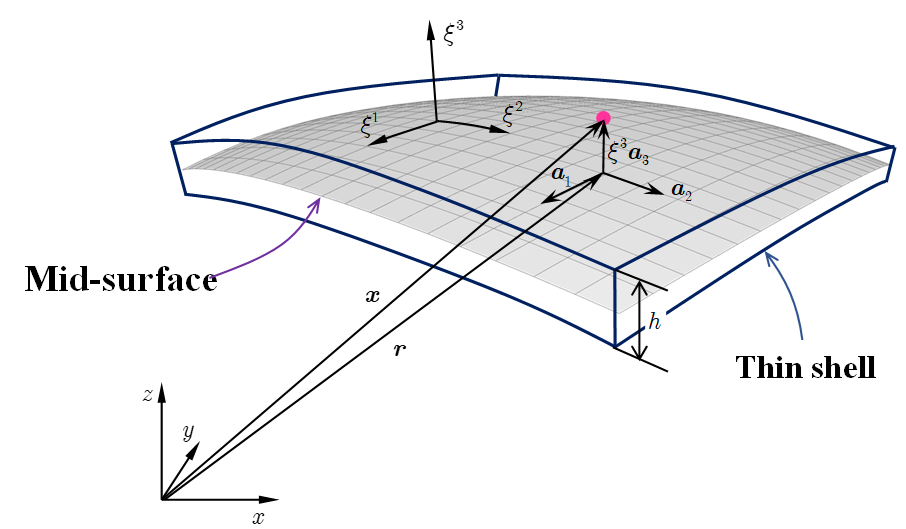
\includegraphics[width=0.7\textwidth]{figures/1}
\caption{Kinematics for thin shell.}\label{fig1}
\end{figure}
in which $\boldsymbol r$ means the position on the mid-surface of shell, and $\boldsymbol a_3$ is corresponding normal direction. For the mid-surface of shell, the in-plane covariant base vector with respect to $\xi^\alpha$ can be derived by a trivial partial differentiation to $\boldsymbol r$:
\begin{equation}
\boldsymbol a_\alpha = \frac{\partial \boldsymbol r}{\partial \xi^\alpha} = \boldsymbol r_{,\alpha}, \alpha  = 1,2
\end{equation}
to provide for a clear expression, the subscript comma denotes the partial differentiation operation with respect to in-plane coordinates $\xi^\alpha$, and the normal vector $\boldsymbol a_3$ can be obtained by the normalized cross product of $\boldsymbol a_{\alpha}$'s as follows:
\begin{equation}
\boldsymbol a_3 = \frac{\boldsymbol a_1 \times \boldsymbol a_2}{\Vert \boldsymbol a_1 \times \boldsymbol a_2 \Vert}
\end{equation}
where $\Vert \bullet \Vert$ is the Euclidean norm operator.

With the assumption of infinitesimal deformation, the strain components with respect to the global contravariant base can be stated as:
\begin{equation}\label{epsilon}
\epsilon_{ij} = \frac{1}{2}(\boldsymbol x_{,i} \cdot \boldsymbol u_{,j} + \boldsymbol u_{,i} \cdot \boldsymbol x_{,j})
\end{equation}
where $\boldsymbol u$ represents the displacement for the shell deformation. To satisfy the Kirchhoff hypothesis, the displacement is assumed to be of the following form:
\begin{equation}\label{u}
\boldsymbol u(\xi^1,\xi^2,\xi^3) = \boldsymbol v(\xi^1,\xi^2) + \boldsymbol \theta(\xi^1,\xi^2) \xi^3
\end{equation}
in which the quadratic and higher order terms are neglected. $\boldsymbol v$, $\boldsymbol \theta$ resperesent the displacement and rotation in mid-surface, respectively.

Subsequently, plugging Eqs. (\ref{x}) and (\ref{u}) into Eq. (\ref{epsilon}) and neglecting the quadratic terms, the strain components can be rephrased as follows:
\begin{subequations}
\begin{align}
\begin{split}
\epsilon_{\alpha\beta} &= \frac{1}{2}(\boldsymbol a_\alpha \cdot \boldsymbol v_{,\beta} + \boldsymbol v_{,\alpha}\cdot \boldsymbol a_\beta) \\ 
&+ \frac{1}{2}(\boldsymbol a_{3,\alpha} \cdot \boldsymbol v_{,\beta} + \boldsymbol v_{,\alpha}\cdot \boldsymbol a_{3,\beta} + \boldsymbol a_\alpha \cdot \boldsymbol \theta_{,\beta} + \boldsymbol \theta_{,\alpha}\cdot \boldsymbol a_\beta)\xi^3 \\
&= \varepsilon_{\alpha\beta} + \kappa_{\alpha\beta}\xi^3
\end{split} \\
\epsilon_{\alpha 3} &= \frac{1}{2}(\boldsymbol a_\alpha \cdot \boldsymbol \theta + \boldsymbol v_{,\alpha}\cdot \boldsymbol a_3) + \frac{1}{2} (\boldsymbol a_3 \cdot \boldsymbol \theta)_{,\alpha}\xi^3 \\ 
\epsilon_{33} &= \boldsymbol a_3 \cdot \boldsymbol \theta
\end{align}
\end{subequations}
where $\varepsilon_{\alpha\beta}$, $\kappa_{\alpha\beta}$ represent membrane and bending strains, respectively, and are given as follows:
\begin{equation}
\varepsilon_{\alpha\beta} = \frac{1}{2}(\boldsymbol a_\alpha \cdot \boldsymbol v_{,\beta} + \boldsymbol v_{,\alpha}\cdot \boldsymbol a_\beta) 
\end{equation}
\begin{equation}\label{kappa1}
\kappa_{\alpha\beta} = \frac{1}{2}(\boldsymbol a_{3,\alpha} \cdot \boldsymbol v_{,\beta} + \boldsymbol v_{,\alpha}\cdot \boldsymbol a_{3,\beta} + \boldsymbol a_\alpha \cdot \boldsymbol \theta_{,\beta} + \boldsymbol \theta_{,\alpha}\cdot \boldsymbol a_\beta)
\end{equation}

In accordance with the Kirchhoff hypothesis, the thickness of shell will not change, and the deformation related with direction of $\xi^3$ will vanish, i.e. $\epsilon_{3i}=0$. Thus, the rotation $\boldsymbol \theta$ can be rewritten as:
\begin{equation}\label{a3}
\epsilon_{3i} = 0 \Rightarrow
\left \{
\begin{split}
&\boldsymbol \theta \cdot \boldsymbol a_\alpha =- \boldsymbol v_{,\alpha} \cdot \boldsymbol a_3 \\
&\boldsymbol \theta \cdot \boldsymbol a_3 = 0
\end{split}
\right .
\Rightarrow \boldsymbol \theta = - \boldsymbol v_{,\alpha} \cdot \boldsymbol a_3 \boldsymbol a^\alpha
\end{equation}
where $\boldsymbol a^\alpha$'s is the in-plane contravariant base vector, $\boldsymbol a^\alpha \cdot \boldsymbol a_\beta = \delta^\alpha_\beta$, $\delta$ is the Kronecker delta function. The detailed derivation of Eq. \ref{a3} can be found in \cite{benzaken2021}.

Furthermore, on substituting Eq. (\ref{a3}) into Eq. (\ref{kappa1}) leads to:
\begin{equation}
\kappa_{\alpha\beta} = (\Gamma^\gamma_{\alpha\beta} \boldsymbol v_{,\gamma} - \boldsymbol v_{,\alpha\beta}) \cdot \boldsymbol a_3 = - \boldsymbol v_{,\alpha}\vert_\beta \cdot \boldsymbol a_3
\end{equation}
in which $\Gamma^\gamma_{\alpha\beta} = \boldsymbol a_{\alpha,\beta} \cdot \boldsymbol a^\gamma$ is namely the Christoffel symbol of the second kind, and $\boldsymbol v_{,\alpha}\vert_\beta$ is the in-plane covariant derivative of $\boldsymbol v_{,\alpha}$, i.e. $\boldsymbol v_{,\alpha}\vert_\beta = \Gamma^\gamma_{\alpha\beta}\boldsymbol v_{,\gamma} - \boldsymbol v_{,\alpha\beta}$.

\subsection{Galerkin weak form for Hu-Washizu principle of complementary energy}
In this study, the Hu-Washizu variational principle of complementary energy \cite{dah-wei1985} was adopted for the development of the proposed analytical approach, the corresponding complementary functional, denoted by $\Pi_C$, is listed as follows:
\begin{equation} \label{functionalc}
\begin{split}
&\Pi_C(\varepsilon_{\alpha\beta},\kappa_{\alpha\beta},N^{\alpha\beta},M^{\alpha\beta}) \\
= &\int_\Omega \frac{h}{2}\varepsilon_{\alpha\beta} C^{\alpha\beta\gamma\eta}\varepsilon_{\gamma\eta}d\Omega 
+ \int_\Omega \frac{h^3}{24}\kappa_{\alpha\beta} C^{\alpha\beta\gamma\eta}\kappa_{\gamma\eta}d\Omega \\
+& \int_\Omega \varepsilon_{\alpha\beta} (N^{\alpha\beta} - h C^{\alpha\beta\gamma\eta} \varepsilon_{\gamma\eta}) d\Omega
+ \int_\Omega \kappa_{\alpha\beta} (M^{\alpha\beta} - \frac{h^3}{12} C^{\alpha\beta\gamma\eta} \kappa_{\gamma\eta}) d\Omega \\
-& \int_{\Gamma_v} \boldsymbol T \cdot \bar{\boldsymbol v} d\Gamma 
+ \int_{\Gamma_\theta} M_{\boldsymbol{nn}} \bar \theta_{\boldsymbol n} d\Gamma - (P \boldsymbol a_3 \cdot \bar{\boldsymbol v})_{\boldsymbol x \in C_w} \\
\end{split}
\end{equation}
where $C^{\alpha\beta\gamma\eta}$'s represent the components of fourth order elasticity tensor with respect to the covariant base and plane stress assumption, and it can be expressed by Young's modulus $E$, Poisson's ratio $\nu$ and the in-plane contravariant metric coefficients $a^{\alpha\beta}$'s, $a^{\alpha\beta} = \boldsymbol a^\alpha \cdot \boldsymbol a^\beta$, as follows: 
\begin{equation}
C^{\alpha\beta\gamma\eta} = \frac{E}{2(1+\nu)}(a^{\alpha\gamma}a^{\beta\eta} + a^{\alpha\eta}a^{\beta\gamma} + \frac{2\nu}{1-\nu} a^{\alpha\beta}a^{\gamma\eta})
\end{equation}
and $N^{\alpha\beta}$, $M^{\alpha\beta}$ represent the components of membrane- and bending- stresses which are given by:
\begin{equation}
N^{\alpha\beta} = hC^{\alpha\beta\gamma\eta}\varepsilon_{\gamma\eta}, \quad
M^{\alpha\beta} = \frac{h^3}{12}C^{\alpha\beta\gamma\eta}\kappa_{\gamma\eta}
\end{equation}

Essential boundaries on the edges and corners denoted by $\Gamma_v$, $\Gamma_\theta$ and $C_v$ are naturally existed in complementary energy functional, and $\bar{\boldsymbol v}$, $\bar \theta_{\boldsymbol n}$ are the corresponding prescribed displacement and normal rotation, respectively. $\boldsymbol T$, $M_{\boldsymbol{nn}}$ and $P$ can be determined by Euler-Lagrange equations of shell problem \cite{benzaken2021} as follows:
\begin{equation}
\boldsymbol T = \boldsymbol T_N + \boldsymbol T_M \; \rightarrow
\begin{cases}
\boldsymbol T_N = \boldsymbol a_\alpha N^{\alpha\beta}n_\beta \\
\boldsymbol T_M = (\boldsymbol a_3 M^{\alpha\beta}s_\alpha n_\beta)_{,\gamma} s^\gamma
+ (\boldsymbol a_3 M^{\alpha\beta})\vert_\beta n_\alpha
\end{cases}
\end{equation}
\begin{equation}
M_{\boldsymbol{nn}} = M^{\alpha\beta}n_\alpha n_\beta
\end{equation}
\begin{equation}
P = -[[M^{\alpha\beta}s_\alpha n_\beta]]
\end{equation}
where $\boldsymbol n = n^\alpha \boldsymbol a_\alpha = n_\alpha \boldsymbol a^\alpha$ and $\boldsymbol s = s^\alpha \boldsymbol a_\alpha = s_\alpha \boldsymbol a^\alpha$ are the outward normal and tangent directions on boundaries. $[[f]]$ is the jump operator defined by:
\begin{equation}
[[f]]_{\boldsymbol x = \boldsymbol x_c} = \lim_{\boldsymbol \epsilon\rightarrow \boldsymbol 0+}(f(\boldsymbol x_c + \boldsymbol \epsilon) - f(\boldsymbol x_c - \boldsymbol \epsilon)), \boldsymbol x_c \in \Gamma
\end{equation}
where $f$ is an arbitrary function on $\Gamma$.

Moreover, the natural boundary conditions should be applied by Lagrangian multiplier method with displacement $\boldsymbol v$ regarded as multiplier. Thus, then the new complementary energy functional namely $\Pi$ is given by:
\begin{equation} \label{functional}
\begin{split}
&\Pi(\boldsymbol v, \varepsilon_{\alpha\beta},\kappa_{\alpha\beta},N^{\alpha\beta},M^{\alpha\beta}) \\
=&\Pi_C(\varepsilon_{\alpha\beta},\kappa_{\alpha\beta},N^{\alpha\beta},M^{\alpha\beta})
+ \int_{\Gamma_M} \theta_{\boldsymbol n} (M_{\boldsymbol{nn}} - \bar M_{\boldsymbol{nn}}) d\Gamma \\
- &\int_{\Gamma_T} \boldsymbol v \cdot (\boldsymbol T - \bar{\boldsymbol T})d\Gamma - \boldsymbol v \cdot \boldsymbol a_3 (P - \bar{P})_{\boldsymbol x \in C_P}
- \int_\Omega \boldsymbol v \cdot (\boldsymbol b - \bar{\boldsymbol b}) d\Omega 
\end{split}
\end{equation}
where $\bar{\boldsymbol T}$, $\bar M_{\boldsymbol{nn}}$ and $\bar P$ are the prescribed traction, bending moment and concentrated force on edges $\Gamma_T$, $\Gamma_M$ and corner $C_P$ respectively. All the specified boundaries meet the following geometric relationships:
\begin{equation}\label{geo}
\begin{cases}
\Gamma=\Gamma_v \cup \Gamma_T \cup \Gamma_\theta \cup \Gamma_M, \quad C = C_v \cup C_P, \\
\Gamma_v \cap \Gamma_T = \Gamma_\theta \cap \Gamma_M = C_v \cap C_P = \varnothing
\end{cases}
\end{equation}
and $\bar{\boldsymbol b}$ stands for the prescribed body force in $\Omega$, $\boldsymbol b$ can be written based on Euler-Lagrange equations \cite{benzaken2021} as:
\begin{equation}
\boldsymbol b = \boldsymbol b_N + \boldsymbol b_M \rightarrow
\begin{cases}
\boldsymbol b_N = (\boldsymbol a_\alpha N^{\alpha\beta})\vert_\beta \\
\boldsymbol b_M = (\boldsymbol a_3 M^{\alpha\beta})\vert_{\alpha\beta}
\end{cases}
\end{equation}

Introducing a standard variational argument to Eq. (\ref{functional}), $\delta \Pi=0$, and considering the arbitrariness of virtual variables, $\delta \boldsymbol v$, $\delta \varepsilon_{\alpha\beta}$, $\delta \kappa_{\alpha\beta}$, $N^{\alpha\beta}$, $M^{\alpha\beta}$ lead to the following weak form:
\begin{subequations}
\begin{equation}\label{w1}
- \int_\Omega h \delta \varepsilon_{\alpha\beta} C^{\alpha\beta\gamma\eta}\varepsilon_{\gamma\eta}d\Omega 
+ \int_\Omega \delta \varepsilon_{\alpha\beta} N^{\alpha\beta} d\Omega = 0
\end{equation}
\begin{equation}\label{w2}
- \int_\Omega \frac{h^3}{12} \delta \kappa_{\alpha\beta} C^{\alpha\beta\gamma\eta}\kappa_{\gamma\eta}d\Omega 
+ \int_\Omega \delta \kappa_{\alpha\beta} M^{\alpha\beta} d\Omega = 0
\end{equation}
\begin{multline}\label{w3}
\int_\Omega \delta N^{\alpha\beta} \varepsilon_{\alpha\beta} d\Omega
- \int_\Gamma \delta \boldsymbol T_N \cdot \boldsymbol v d\Gamma 
+ \int_\Omega \delta \boldsymbol b_N \cdot \boldsymbol v d\Omega \\
+ \int_{\Gamma_v} \delta \boldsymbol T_N \cdot \boldsymbol v d\Gamma 
= \int_{\Gamma_v} \delta \boldsymbol T_N \cdot \bar{\boldsymbol v} d\Gamma 
\end{multline}
\begin{multline}\label{w4}
\int_\Omega \delta M^{\alpha\beta} \kappa_{\alpha\beta} d\Omega 
- \int_\Gamma \delta M_{\boldsymbol{nn}} \theta_{\boldsymbol n}d\Gamma
+ \int_\Gamma \delta \boldsymbol T_M \cdot \boldsymbol v d\Gamma
+ (\delta P \boldsymbol a_3 \cdot \boldsymbol v)_{\boldsymbol x \in C}
+ \int_\Omega \delta \boldsymbol b_M \cdot \boldsymbol v d\Omega \\
+ \int_{\Gamma_\theta} \delta M_{\boldsymbol{nn}} \theta_{\boldsymbol n}d\Gamma
- \int_{\Gamma_v} \delta \boldsymbol T_M \cdot \boldsymbol v d\Gamma
- (\delta P \boldsymbol a_3 \cdot \boldsymbol v)_{\boldsymbol x \in C_v} \\ =
\int_{\Gamma_\theta} \delta M_{\boldsymbol{nn}} \bar{\theta}_{\boldsymbol n}d\Gamma
- \int_{\Gamma_v} \delta \boldsymbol T_M \cdot \bar{\boldsymbol v} d\Gamma
- (\delta P \boldsymbol a_3 \cdot \bar{\boldsymbol v})_{\boldsymbol x \in C_v}
\end{multline}
\begin{multline}\label{w5}
\int_{\Gamma} \delta \theta_{\boldsymbol n} M_{\boldsymbol{nn}} d\Gamma
    - \int_\Gamma \delta \boldsymbol v \cdot \boldsymbol T d\Gamma 
    - (\delta \boldsymbol v \cdot \boldsymbol a_3 P)_{\boldsymbol x \in C}
    + \int_\Omega \delta \boldsymbol v \cdot \boldsymbol b d\Omega \\
    - \int_{\Gamma_\theta} \delta \theta_{\boldsymbol n} M_{\boldsymbol{nn}} d\Gamma
    + \int_{\Gamma_v} \delta \boldsymbol v \cdot \boldsymbol T d\Gamma 
    + (\delta \boldsymbol v \cdot \boldsymbol a_3 P)_{\boldsymbol x \in C_v}
    = - \int_{\Gamma_T} \delta \boldsymbol v \cdot \bar{\boldsymbol t} d\Gamma - \int_\Omega \delta \boldsymbol v \cdot \bar{\boldsymbol b} d\Omega
\end{multline}
\end{subequations}
where the geometric relationships of Eq. (\ref{geo}) is used herein.
